\section{Practicality of Covert Communication}
\label{sec:study}

In this section, we perform a study to demonstrate the practicality of data 
transfer using the lambda covert channels discovered with our co-residence detector.  
The amount of information that can be transferred depends on two factors: 1) the 
capacity of each channel and 2) the number of co-resident clusters of lambdas, 
or rendezvous points, that materialize during the attack.  We first produce an estimate on the
capacity of the covert channels established, and then examine the co-residence
density in various AWS regions to understand the number of rendezvous points and
factors that affect it.

\subsection{Covert Channel Capacity}


Once co-residence between any two lambas is established, the attacker can then
use the same memory bus hardware to perform covert communication. Wu et
al.~\cite{wuusenix2012}, who first introduced covert channel based on this
hardware channel, also presented an efficient and error-free communication
protocol targeting cloud-based platforms like VMs.  While such a protocol should
theoretically work for lambdas, extending it is beyond the scope of this work.
We do, however, use a much simpler (albeit more inefficient) protocol to report
a conservative estimate of the capacity of each covert channel.

Our protocol for data transfer uses the bus contention in the same way as the co-residence
detector in section \ref{sec:method:impl} to send and receive bits and perform clock
synchronization. However, now that we can use our co-residence detector to identify
lambdas on a machine and target the two that we wish to label as the sender and
receiver, we are not concerened about noise from multiple receivers, and as such
can allow the receiver to sample continuously (section \ref{sec:method:listen:freq}) 
and sample for extremely small duration (milliseconds instead of seconds). While we want the
sampling duration to be as small as possible (in order to increase the rate of
bits transferred), the chances of erasures or errors also increases as the
sender and receiver may get descheduled during this time. 

To demonstrate this, we launched hundreds of 3 GB lambdas on AWS and use our
co-residence detector to establish tens of covert channels. We then send data
over these channels at various bitrates and record the error ratio (for
byte-sized data segments). Figure~\ref{fig:channel} shows the mean error ratio
at 50\% and 95\% one-sided confidence intervals, both of which increase with the bitrate.


To correct these errors, we use Reed-Solomon coding, a block-based error correction 
code that is suitable for burst-errors caused by descheduling~\cite{wuusenix2012}. 
However, error correction comes with an overhead; With byte-sized symbols,
Reed-Solomon requires twice as many parity bytes as there are errors to correct. 
So, for each bitrate, we must compute
effective bitrate by subtracting the overhead of error correction bytes.
%required to correct its corresponding 95\% error. 
From Figure~\ref{fig:channel}, we can see that effective bitrate rises to a
maximum of over 200 bits per second (bps) (at 500 bps raw rate) before falling
again due to high error rate. We confirmed this by sending Reed-Solomon encoded
data over the covert channels at this rate and observed near-zero data
corruption. Thus, we conclude that, by a conservative estimate, we can safely
send data across each of these covert channels at a rate of ~200 bps.



\begin{figure}[!t]
  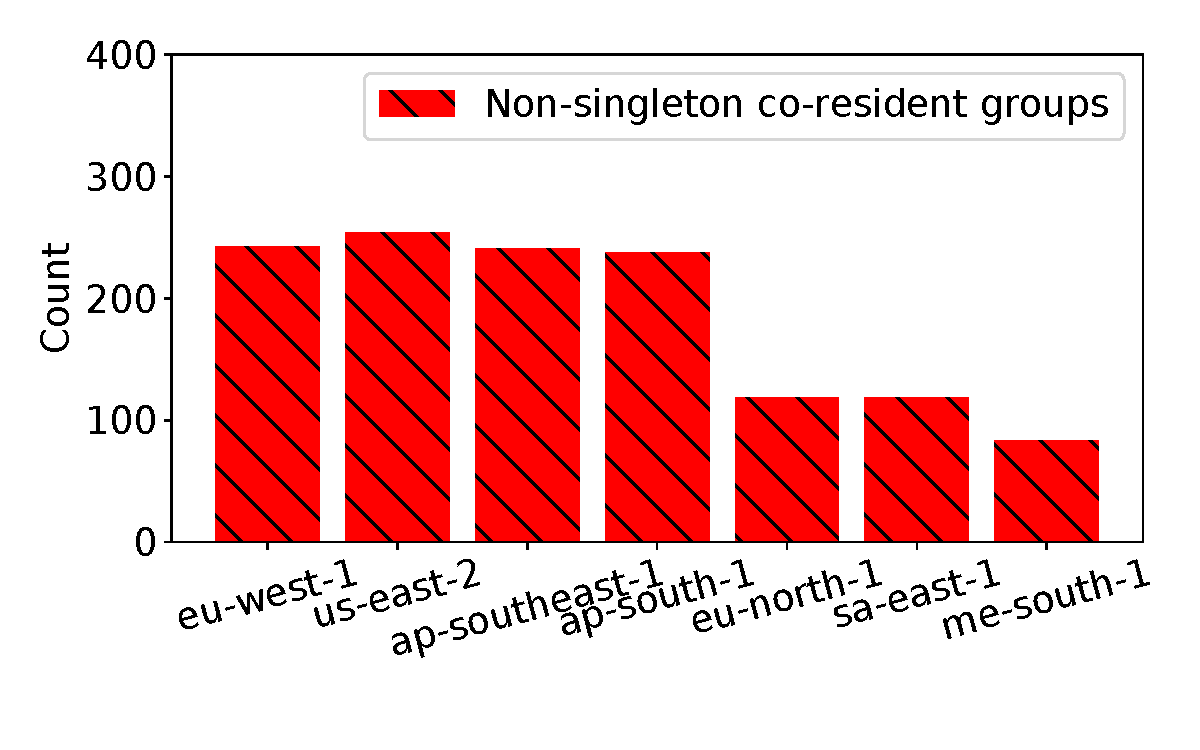
\includegraphics[width=.99\linewidth]{fig/clusters.pdf}
  \caption{This figure shows the average number of lambdas per server i.e., the co-residence 
  density seen in various AWS regions for the runs shown in Figure~\ref{fig:awsregions}. 
  The ample co-residence across regions demonstrates the practicality of establishing 
  covert channels with lambdas in these regions.
\label{fig:clusters}}
\end{figure}


\subsection{Covert Channel Density}
Finally, we present measurements on covert channel density on AWS using our
co-residence detector, and discuss the factors that may affect this density.  As
we discussed in section \ref{sec:motivation}, each co-resident group of lambdas 
represent an individual server in the cloud and hence can enable an independent 
covert channel whereever the group has more than two lambdas. So we attempt to answer 
the following question: assuming that the user launches a number of
(sender and receiver) lambdas at a specific point in time, what is the expected
number of such co-resident groups (with two or more lambdas) that they might see? 
We deploy a large number of lambdas on various AWS regions and report the co-residence 
density, that is, the average number of such co-residence groups. The higher the 
co-residence density, the easier it is for the user
to ultimately establish covert channels with lambdas, and the more information
they can send. Unless specified otherwise, all the experiments discussed in this
section are performed with 1.5 GB lambdas and executed successfully with
\textbf{zero error} in co-residence detection.


\begin{figure*}[!t]
    \begin{subfigure}{.5\textwidth}
      \centering
      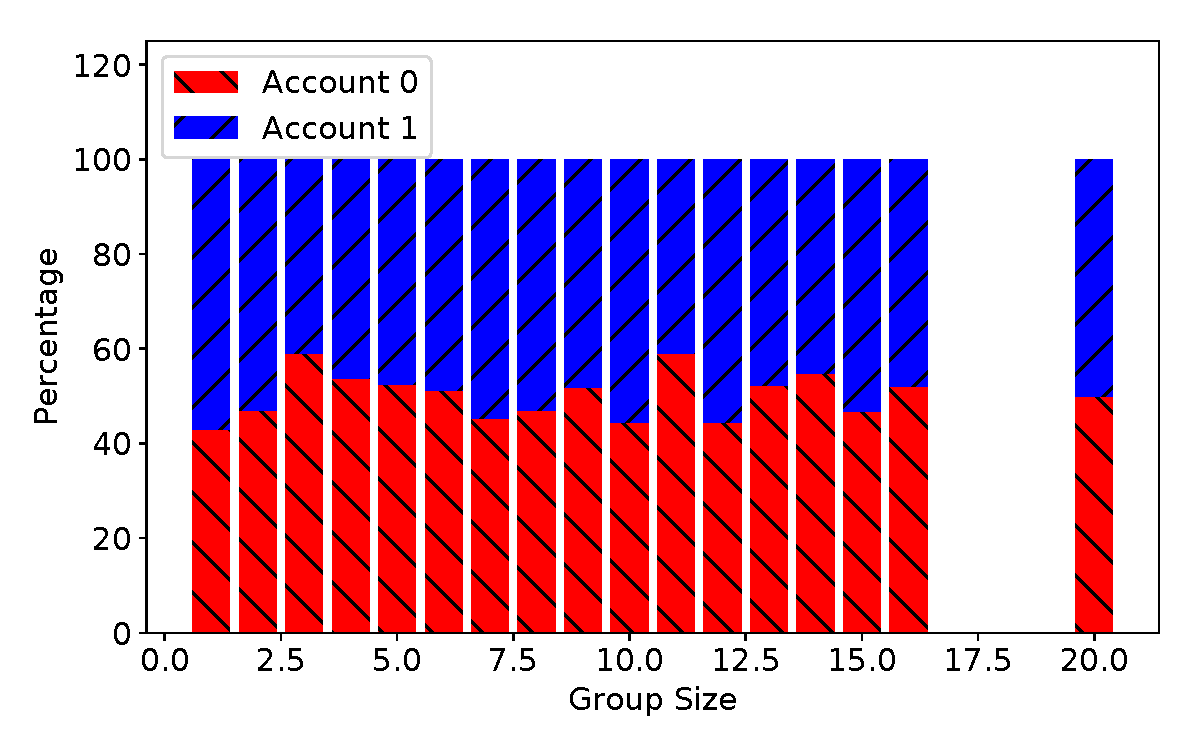
\includegraphics[width=.99\linewidth]{fig/different-accounts.pdf}
    %   \caption{1a}
    %   \label{fig:sfig1}
    \end{subfigure}%
    \begin{subfigure}{.5\textwidth}
      \centering
      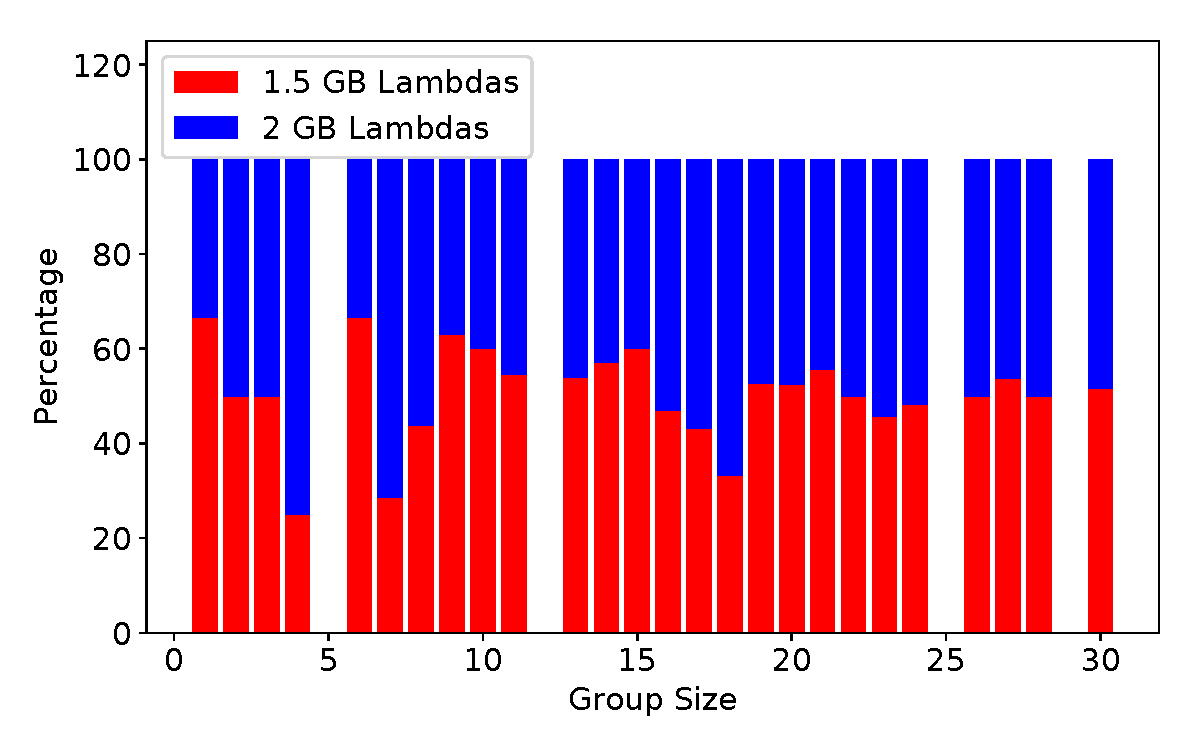
\includegraphics[width=.99\linewidth]{fig/different-sizes.pdf}
    %   \caption{1b}
    %   \label{fig:sfig2}
    \end{subfigure}

    \caption{The left plot shows the breakdown of co-resident groups (of varying
    sizes) of lambdas by two different accounts in an experiment of 1000
    lambdas, where 500 lambdas are launched from each account. The uniformity of
    the split suggests that the lambda scheduler might be invariant to the
    account the lambdas are launched from. Similar results are shown for
    different lambda sizes in the right plot. }
    \label{fig:factors}
\end{figure*}


\subsubsection{Across AWS regions}  
We execute our co-residence detector with 1000 1.5 GB Lambdas in various AWS
regions. Figure~\ref{fig:awsregions} comprises multiple plots depicting
the co-resident groups per region, with each bar indicating the fraction of
lambdas that detected a certain number of neighbors (i.e., that belong to a
co-resident group of a certain size). Plots that skew to the right indicate a
higher co-residence density when compared to the plots skewed to the left. 
We note that, in most regions, almost
all lambdas recognize at least one neighbor (indicated by smaller or
non-existent first bar in each plot). We hypothesize that the co-residence
density is (inversely) dependent on the total number of servers and the lambda
activity in the region, both of which can be assumed to be lower in newer AWS
regions resulting in higher co-residence density in those regions. 
Figure~\ref{fig:density} shows the total number of co-resident groups with 
two or more lambdas, each of which can be an independent covert channel. 
The ample co-residence in general ac  ross all the
regions shows that lambdas provide a fertile ground for covert channels.
%We note that the largest co-resident group on a single machine was comprised of 25 lambdas. 


\subsubsection{Other factors}
We also examine how co-residence is affected by various launch strategies that
the user may use, like deploying lambdas from multiple AWS accounts and
different lambda sizes. In particular, we wish to determine if we our mechanism
exhibits different results when: 1) the user deploys sender lambdas and receiver
lambdas on two separate accounts (normally the case with covert channels) and 2)
the senders and receivers are created with different lambdas sizes.  To answer
these questions, we run an experiment with 1000 lambdas of which we launch 500
lambdas from one account (senders) and 500 from other deployed in a random
order. The co-residence observed was comparable to the case where all the
lambdas were launched from one account. In the left subfigure of
Figure~\ref{fig:factors}, we show the breakdown of co-resident group of lambdas
of each size among the two accounts.  We can see that among the co-resident
groups of all sizes, roughly half of lambdas came from either account. This suggests 
that lambda scheduler could be agnostic to the accounts the lambdas were launched
from. We see similar results for different lambda sizes, as shown in the right
subfigure of Figure~\ref{fig:factors}.

%From our experiments, we also observe that co-residence density in a region
%barely changes during course of the day or the week (data not shown
%in any figure \todo{is this okay?}).  This gives the user the freedom to utilize this
%technique at any time and expect similar results.
